
\documentclass{article}
\usepackage[final]{nips_2017}
\usepackage[utf8]{inputenc}
\usepackage{graphicx, float}
\graphicspath{ {images1/} }
\usepackage{babel,blindtext}

\title{Generalised Reinforced learning algorithms for games by self play}
\author{
    Abhinav (6047704638) \And
    Kaladhar (7761016469) \And
    Pallavi (2611733530)
}
\begin{document}
\maketitle

\begin{abstract}
  Mastering any board game is one of the most widely researched AI problems. The strongest programs have been recently combined neural networks with reinforcement learning to achieve very good performance against human opponent. However these algorithms are not generalized enough to be applied to other problems/games. This can be improved using a single and more generalized AlphaZero Algorithm that can achieve superhuman performance in various domains.
\end{abstract}

\section{Introduction}
    Much progress towards artificial intelligence has been made using supervised learning systems that are trained to replicate the decisions of human experts. However, expert data sets are often expensive, unreliable or simply unavailable. Even when reliable data sets are available, they may impose a ceiling on the performance of systems trained in this manner. By contrast, reinforcement learning systems are trained from their own experience, in principle allowing them to exceed human capabilities, and to operate in domains where human expertise is lacking.

    Alpha Zero(1) is one of a kind algorithm in this field which got lot of attention in the year 2017. Alpha Zero has had success in beating all other systems in board games, by using Neural Networks and MCTS( Monte Carlo Tree Search) for self-play. We made use of these algorithms to build games like TIC-TAC-TOE and Checkers.


\section{Problem Description}


Though games are easy to  formulate they are difficult to master for a machine, this being the reason it has been a popular area of artificial intelligence research for a long time. For decades, game developer have attempted to create the agent with simulate intelligence, specifically, to build the AI player who can learn the game based on its gaming experience, rather than merely following one fixed strategy. The dynamic programming could solve the problem with relative small number of states and simple underlying random structure, but not the complex one.

Most of the other models achieved good performance by using alpha-beta search engine with many domain specific adaptations. Instead of an alpha-beta search with domain-specific enhancements, AlphaZero uses a general purpose Monte-Carlo tree search (MCTS) algorithm. Each search consists of a series of simulated games of self-play that traverse a tree from root sroot to leaf. Each simulation proceeds by selecting in each state s a move a with low visit count, high move probability and high value (averaged over the leaf states of simulations that selected a from s) according to the current neural network f$\theta$.
The search returns a vector $\pi$ representing a probability distribution over moves, either proportionally or greedily with respect to the visit counts at the root state.

The neural network parameters in AlphaZero are trained by self-play reinforcement learning. The parameters are initialized randomly. AlphaGo Zero estimates and optimises the probability of winning, assuming binary win/loss outcomes. AlphaZero instead estimates and optimises the expected outcome, taking account of draws or potentially other outcomes.


\section{Methods Used}

\subsection{Monte-Carlo Tree Search}\footnote[1]{Environment adapted from             https://github.com/kaladharusc/DeepReinforcementLearning}
The focus of Monte Carlo tree search is on the analysis of the most promising moves, expanding the search tree based on random sampling of the search space. The application of Monte Carlo tree search in games is based on many playouts. In each playout, the game is played out to the very end by selecting moves at random. The final game result of each playout is then used to weight the nodes in the game tree so that better nodes are more likely to be chosen in future playouts.

\subsection{Policy and Value Network}
    Both Policy and Value are determined by the same network.The heads (output layer) are different for the Network. The value function is a continuous-valued function between [-1,1]. Also, Policy network provides the Probability for the next best move.This makes the network robust as the loss function is applied to the ‘common network’ and the respective heads.SGD is used to reduce the loss for each batch.

    Residual Networks are used to achieve more depth in terms of layers.The utilization of RN’s allowed for 20 RN’s.Vanishing Gradients problem is reduced and training error does not increase as the input takes a shortcut with the help of an identity mapping.The actual residual block consists of two CNN’s instead of a Dense Layer.

    In each simulation of our algorithm, the best model play a number of episodes (30 in  the current experiments) of self-play using MCTS. The resulting training examples is of the form (s(t), ~π(t), z(t)).

    Then, the current best is updated  neural network using the new training examples, to get a new neural network. We then play the old and new networks against each other for a number of games (30 in our experiments). If the new network wins more than a set threshold number of times, the network is updated and continue with the next iteration, resetting the MCTS tree. Else, we continue with the old network and the old MCTS tree, and conduct another iteration to augment our training examples further.

    \blindtext
    \begin{figure}[H]
        \centering
        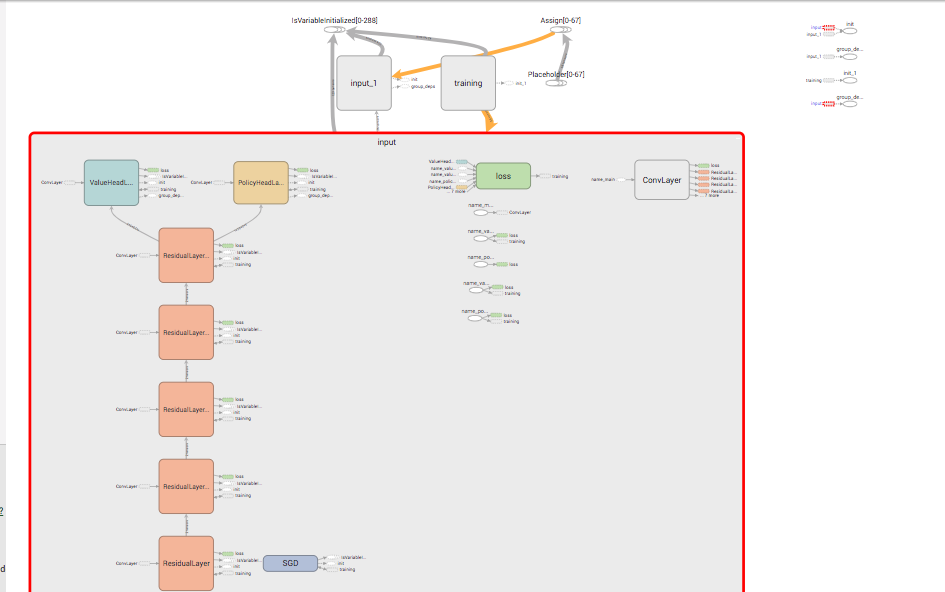
\includegraphics[width=\textwidth, scale=0.5]{tensorflow.png}
        \caption{Neural Network Architecture}
        \label{fig:my_label}
    \end{figure}


\section{Data Description}

\begin{enumerate}
    \item Consists of set of domain rules explaining the game.
        \begin{itemize}
            \item 1 for player1 and -1 for player2
            \item 1 if current player wins, -1 if current player looses, 0 if its a draw game.
        \end{itemize}
    \item The state space to represent the players of the game and also the spatial
representation the board/screen.

    \item The decision for the next move is calculated on the fly using neural networks.
        \begin{itemize}
            \item Using MCTS and RNN, based on value and policy network, decision is made maximizing the winning chances.
        \end{itemize}
\end{enumerate}

\section{Results}
\subsection{Tic-Tac-Toe}

Below is the games we developed for tic-tac-tow. We trained the model for 1 hr with 30 Episodes and 30 MCTS simulation for each move and found the it was able to achieve human level performance very quickly and able to beat human in 5 out of 10 games, and 3 games were draw.
\begin{figure}[H]
    \centering
    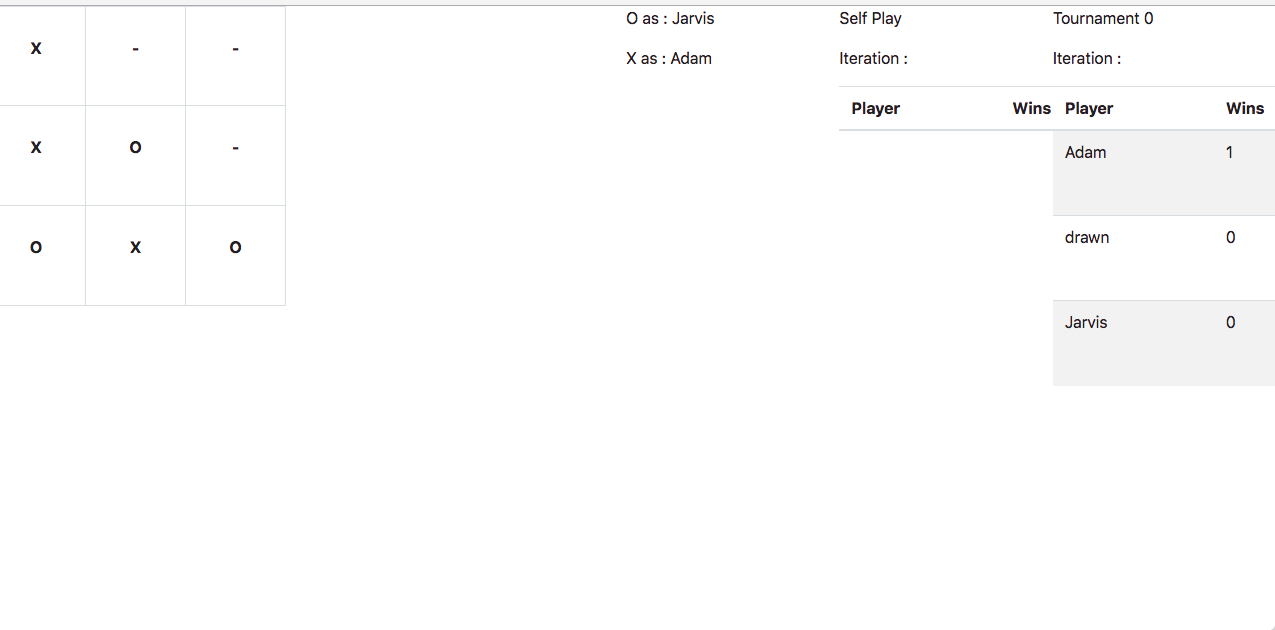
\includegraphics[width=\textwidth,scale=0.5]{tictactoe.png}
    \caption{Tic-Tac-Toe}
    \label{fig:my_label}
\end{figure}

This was easy to train and easy to model the rules of the game, so that we moved to checkers game.

\subsection{Checkers}
\subsubsection{Lessons learned}
It is much harder game state to represent and to model the winning moves and winning state. We handled the problem step by step. Below is the game we implemented. We have used sockets to let the humans play against best model we trained for 2 hrs. Trained model was able to make winning moves by itself without any input from human. Trained model was able to beat human in 3 out of 5 games.

Actions space is different from game state.
    \begin{enumerate}
        \item In our game Game state is : 8 X 8
        \item Actions Space is 84 ( i.e there are 85 ways player can play ). Then we have to rever positon for other     player.
        \item Then for every game, we filter out allowed action based on checkers game rules.
    \end{enumerate}

\begin{figure}[H]
    \centering
    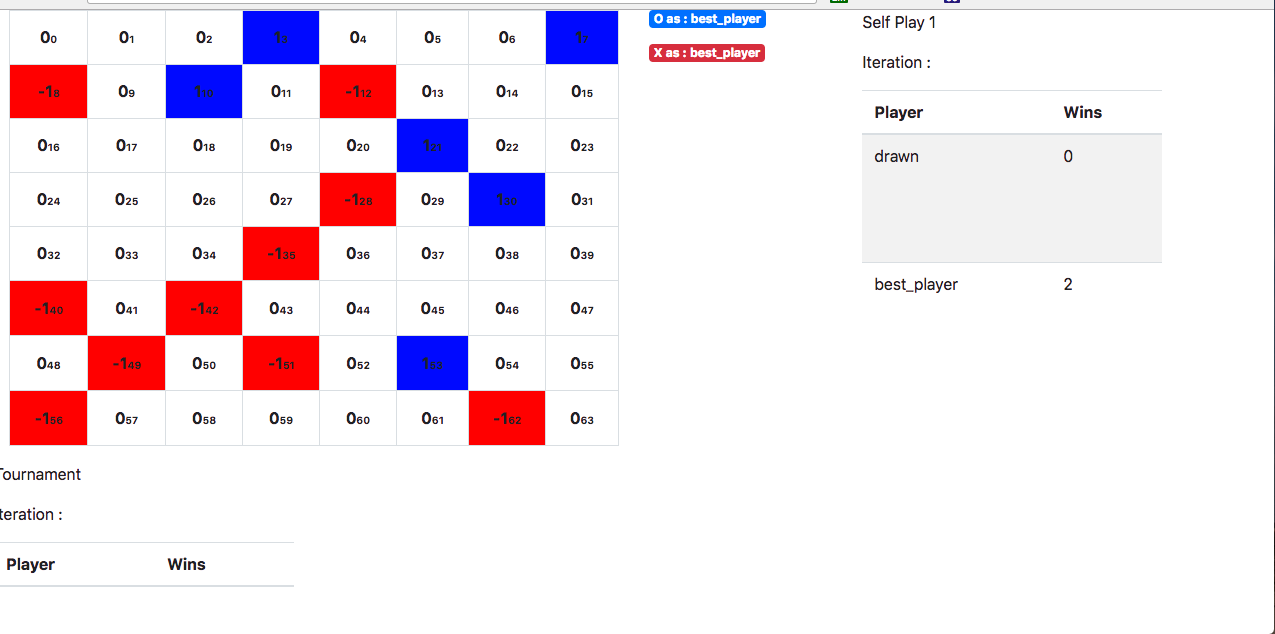
\includegraphics[width=\textwidth,scale=0.1,]{checkers.png}
    \caption{Checkers}
    \label{fig:my_label}
\end{figure}


\subsection{Losses}

We have trained the model using different network sizes.Below are the graphs. Though we can see that loss is decreased for minimal complex networks, they were not able to train themselves to win the game, most of the low complex model were drawn games. Once we move the architecture to 6 hidden layers and 75 filters with 4x4 size, the model started to win games more often, though loss is decreasing slowly.

    \begin{figure}[!htb]
        \centering
        \minipage{0.32\textwidth}
            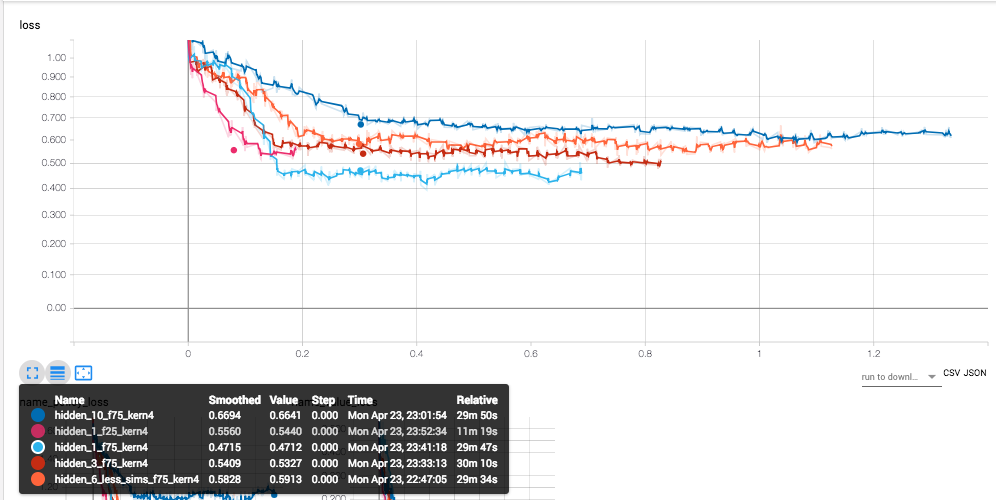
\includegraphics[width=\linewidth]{loss.png}
            \caption{Loss}
        \endminipage\hfill
        \minipage{0.32\textwidth}
            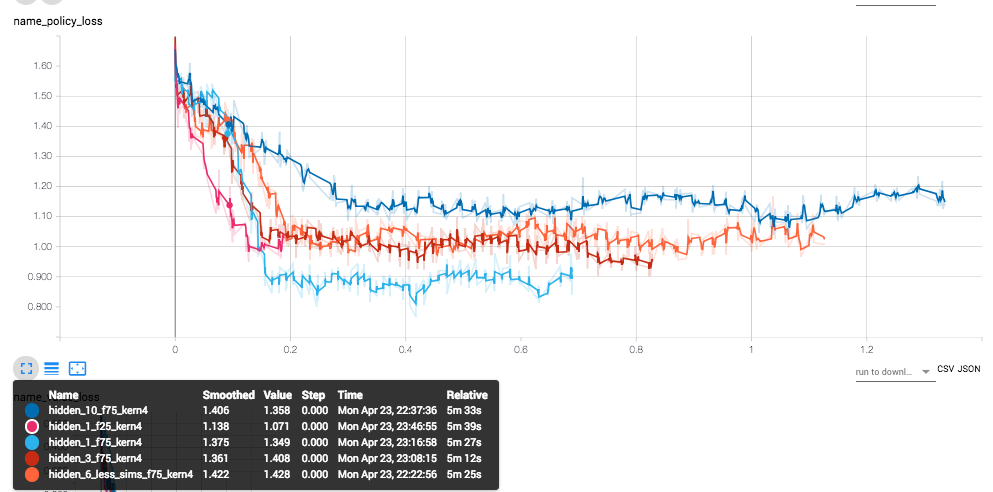
\includegraphics[width=\linewidth]{name_policy_loss.png}
            \caption{Policy Loss}
        \endminipage\hfill
        \minipage{0.32\textwidth}
            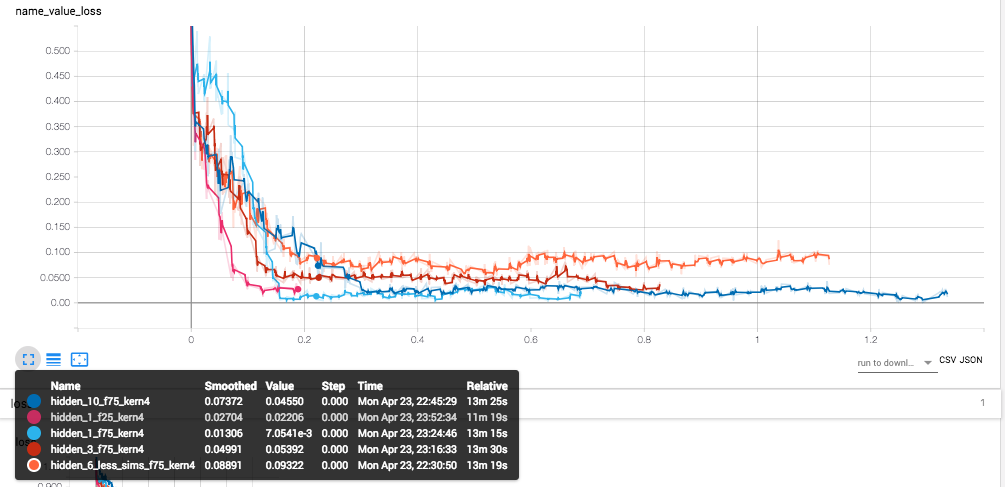
\includegraphics[width=\linewidth]{name_value_loss.png}
            \caption{Value Loss}
        \endminipage\hfill
    \end{figure}

% 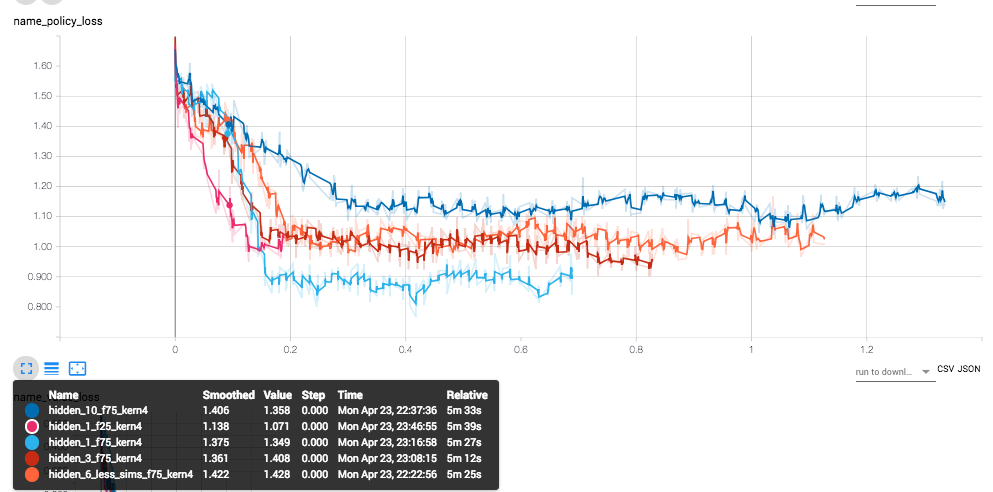
\includegraphics[width=\textwidth, scale=0.5]{name_policy_loss.png}
% 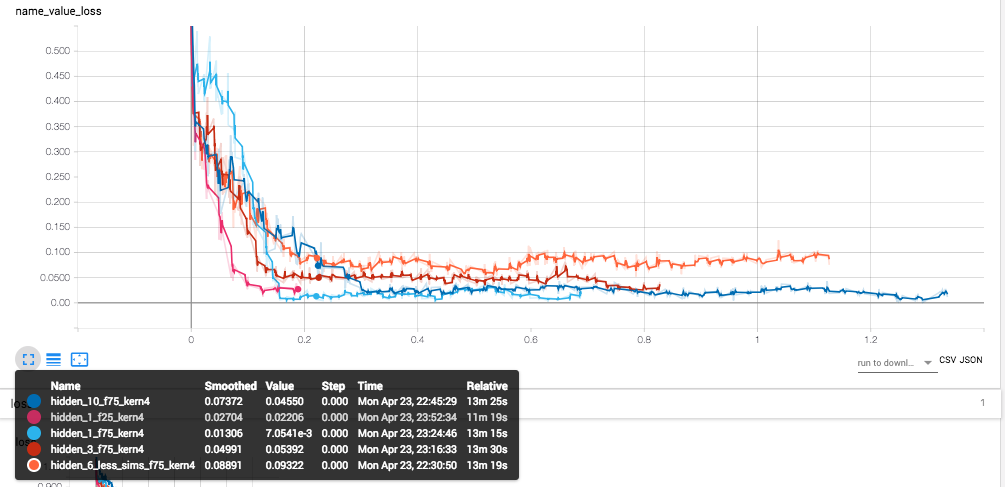
\includegraphics[width=\textwidth, scale=0.5]{name_value_loss.png}


\section{Future work}
\begin{itemize}
    \item The goal is to use the generalized RL algorithm to other problems/games.
    \item Train the checkers game model with all the ruls of the game like multi kill in one move.
    \item Then extend the project to train other games like chess and Backgammon.
\end{itemize}

\section{Conclusions}
We implemented an agent that learns itself to play tic-tac-toe and checkers without any human knowledge. The model we trained beats more than 80\% of times in tic-tac toe and more than 60\% of times in checkers. The time taken to make move is less than a second of checkers and less than 100ms for tic-tac-toe. As seen in section 3 our project is generic enough in its implmentaion to extent it to other sum zero board games.

The original implementation by DeepMind (Silver et
al. 2017b) uses orders of magnitude more raw computational
power on industry hardware (4TPUs, 64GPUs,
and 19CPUs, for several days). In our work, we show
that it is possible to train similar networks on commodity
hardware for smaller problems.


\section*{References}

[1] David Silver, Thomas Hubert \ \& Julian Schrittwieser. {\it Mastering Chess and Shogi by      Self-Play with a General Reinforcement Learning Algorithm. } December 2017
    (\url{https://arxiv.org/pdf/1712.01815.pdf})
    
[2] \url{https://medium.freecodecamp.org/explained-simply-how-an-ai-program-mastered-the-ancient-game-of-go-62b8940a9080}

[3] \url{https://medium.com/applied-data-science/how-to-build-your-own-alphazero-ai-using-python-and-keras-7f664945c188}


\end{document}